\documentclass[a4,useAMS,usenatbib,usegraphicx,12pt]{article}
%External Packages and personalized macros
%=========================================================================
%		EXTERNAL PACKAGES
%=========================================================================
\usepackage[round]{natbib}
\usepackage[margin=3cm]{geometry}
\usepackage{hyperref}
\usepackage{times}
\usepackage{amsmath} 
\usepackage{amssymb}
\usepackage{graphicx}
\usepackage{array, xcolor, lipsum, bibentry}
\usepackage[nottoc, notlof, notlot]{tocbibind}

\definecolor{lightgray}{gray}{0.8}
\newcolumntype{L}{>{\raggedleft}p{0.14\textwidth}}
\newcolumntype{R}{p{0.8\textwidth}}
\newcommand\VRule{\color{lightgray}\vrule width 0.5pt}

\usepackage{booktabs}% http://ctan.org/pkg/booktabs
\newcommand{\tabitem}{~~\llap{\textbullet}~~}

%=========================================================================
%		INTERNAL MACROS
%=========================================================================
% To highlight comments 
\definecolor{red}{rgb}{1,0.0,0.0}
\newcommand{\red}{\color{red}}
\definecolor{darkgreen}{rgb}{0.0,0.5,0.0}
\newcommand{\SRK}[1]{\textcolor{darkgreen}{\bf SRK: \textit{#1}}}
\newcommand{\SRKED}[1]{\textcolor{darkgreen}{\bf #1}}

\newcommand{\LCDM}{$\Lambda$CDM~}
\newcommand{\beq}{\begin{eqnarray}}  
\newcommand{\eeq}{\end{eqnarray}}  
\newcommand{\zz}{$z\sim 3$} 
\newcommand{\apj}{ApJ}  
\newcommand{\apjs}{ApJS}  
\newcommand{\apjl}{ApJL}  
\newcommand{\aj}{AJ}  
\newcommand{\mnras}{MNRAS}  
\newcommand{\mnrassub}{MNRAS accepted}  
\newcommand{\aap}{A\&A}  
\newcommand{\aaps}{A\&AS}  
\newcommand{\araa}{ARA\&A}  
\newcommand{\nat}{Nature}  
\newcommand{\physrep}{PhR}
\newcommand{\pasp}{PASP}    
\newcommand{\pasj}{PASJ}    
\newcommand{\avg}[1]{\langle{#1}\rangle}  
\newcommand{\ly}{{\ifmmode{{\rm Ly}\alpha}\else{Ly$\alpha$}\fi}}
\newcommand{\hMpc}{{\ifmmode{h^{-1}{\rm Mpc}}\else{$h^{-1}$Mpc }\fi}}  
\newcommand{\hGpc}{{\ifmmode{h^{-1}{\rm Gpc}}\else{$h^{-1}$Gpc }\fi}}  
\newcommand{\hmpc}{{\ifmmode{h^{-1}{\rm Mpc}}\else{$h^{-1}$Mpc }\fi}}  
\newcommand{\hkpc}{{\ifmmode{h^{-1}{\rm kpc}}\else{$h^{-1}$kpc }\fi}}  
\newcommand{\hMsun}{{\ifmmode{h^{-1}{\rm {M_{\odot}}}}\else{$h^{-1}{\rm{M_{\odot}}}$}\fi}}  
\newcommand{\hmsun}{{\ifmmode{h^{-1}{\rm {M_{\odot}}}}\else{$h^{-1}{\rm{M_{\odot}}}$}\fi}}  
\newcommand{\Msun}{{\ifmmode{{\rm {M_{\odot}}}}\else{${\rm{M_{\odot}}}$}\fi}}  
\newcommand{\msun}{{\ifmmode{{\rm {M_{\odot}}}}\else{${\rm{M_{\odot}}}$}\fi}}  
\newcommand{\lya}{{Lyman$\alpha$~}}
\newcommand{\clara}{{\texttt{CLARA}}~}
\newcommand{\rand}{{\ifmmode{{\mathcal{R}}}\else{${\mathcal{R}}$ }\fi}}  


%MY COMMANDS #############################################################
\newcommand{\sub}[1]{\mbox{\scriptsize{#1}}}
\newcommand{\dtot}[2]{ \frac{ d #1 }{d #2} }
\newcommand{\dpar}[2]{ \frac{ \partial #1 }{\partial #2} }
\newcommand{\pr}[1]{ \left( #1 \right) }
\newcommand{\corc}[1]{ \left[ #1 \right] }
\newcommand{\lla}[1]{ \left\{ #1 \right\} }
\newcommand{\bds}[1]{\boldsymbol{ #1 }}
\newcommand{\oiint}{\displaystyle\bigcirc\!\!\!\!\!\!\!\!\int\!\!\!\!\!\int}
\newcommand{\mathsize}[2]{\mbox{\fontsize{#1}{#1}\selectfont $#2$}}
\newcommand{\eq}[2]{\begin{equation} \label{eq:#1} #2 \end{equation}}
\newcommand{\lth}{$\lambda_{th}$ }
%#########################################################################

\setlength\parindent{0pt}
 
\title{{\textbf{Research Proposal for a Master Thesis in Physics}}\\ 
				Verifying the VPH scheme in Galaxy Formation\\ 
				\color{black}\rule{15cm}{0.5mm}}
\author{Sebastian Bustamante Jaramillo}
\date{}
  
\begin{document}
\maketitle
\begin{center}
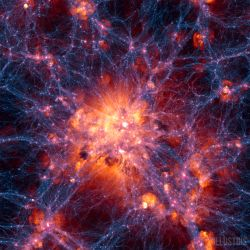
\includegraphics[trim = 0mm 3.5cm 0mm 3.0cm, clip, keepaspectratio=true,
width=0.7\textheight]{Presentation1.png}
\tiny{Time evolution of a gas cloud in a supersonic wind using a \VPH\ scheme.
Taken from \citep{Hess10}}
\end{center}
\tableofcontents
 
\newpage 

%============================================================================== 
\section{General Information}
\small
\subsection*{Information of the Student}
\begin{tabular}{L!{\VRule}R}
\bf Name		& Sebastian Bustamante Jaramillo\\
\bf Degree		& B.Sc. in Physics, Universidad de Antioquia (2013)\\
\bf E-mail 1	& macsebas33 \textit{at} gmail.com (personal)\\
\bf E-mail 2	& sebastian.bustamante \textit{at} udea.edu.co (academic)\\
\end{tabular}

\vspace{10pt}

More detailed information of the applicant can be found here \url{http://goo.gl/BPZGzK}

\vspace{15pt}  

\subsection*{Information of the Project}
\begin{tabular}{L!{\VRule}R}
\bf Title		& \bf Verifying the VPH scheme in Galaxy Formation\\
\bf Field		& Cosmology, Astrophysics, Physical Sciences \\
\bf Advisor 1	& Professor Juan Carlos Munoz-Cuartas. Universidad de Antioquia, Colombia.\\
\bf University	& Universidad de Antioquia, Master of Physics program \\
\bf Time Frame	& 2 years \\
\end{tabular}
\normalsize
%==============================================================================

%==============================================================================
\section{Abstract}
%==============================================================================

The complex processes involved in some astrophysical scenarios like galaxy 
formation, makes necessary the use of numerical approaches for a deeper 
understanding. We are especially concerned here with hydrodynamical schemes for
solving the dynamics of a gas for galaxy formation in a cosmological setup.
Two families of hydro-solvers have been widely used in astrophysics, namely a
family of Lagrangian methods, where the fluid evolution is followed by means of
a set of sampling particles, and a second family of mesh-based methods in 
which the evolution is performed over a grid. Although these methods describe 
well several situations, they also exhibit some weaknesses that make them poor 
suitable for solving full hydrodynamical cosmological simulations. Recently, a 
new hydro-solver was implemented into the \AREPO\ code, in principle solving 
many of the weaknesses of the classic schemes and exploiting their strengths. 
Despite of the high accuracy achieved, the price to pay for this is an 
increased complexity in code development and design, making the reproducibility 
very hard, in addition to a prohibitive computing time when limited 
computational resources are available. We shall explore a modification of the 
\textit{Smoothed Particle Hydrodynamic} \SPH\ scheme based on Voronoi 
tessellations for field estimation, i.e. the \textit{Voronoi Particle 
Hydrodynamic} \VPH. This new approach improves greatly the accuracy of classic 
Lagrangian methods, but keeping a reasonable computing time. We shall compare 
here the physical accuracy and the computational efficiency of \VPH\ with 
\SPH and \AREPO.

\newpage


%==============================================================================
\section{Introduction}
%==============================================================================
As we understand more deeply the physical processes involved in astrophysical 
phenomena, it becomes necessary to compute complex interactions of an ever 
increasing number of single components. Some prominent examples include 
the large-scale Universe, galaxy evolution, stellar interior, star formation 
and protoplanetary disk dynamics. A common aspect of these examples is that all 
of them can be regarded basically as a fluid mechanic problem.

\

Although the development of analytical approaches has demonstrated to be a
valuable resource for studying these processes, their increasing complexity 
makes it necessary to invoke numerical solutions as a more feasible alternative.
For this purpose, two different families of hydrodynamics solvers has been 
explored and widely used by the astrophysical community. First, a family of 
Lagrangian techniques (e.g. \textit{Smoothed Particle Hydrodynamics} 
\SPH\ \citep{Lucy77,Gingold77}, \textit{Voronoi Particle Hydrodynamics} \VPH\ 
\citep{Hess10}), and a second family of Eulerian techniques (e.g.
\textit{Adaptive Mesh Refinement} \texttt{AMR} \citep{Berger89}).

\

Due to the their Lagrangian character, techniques like \SPH\ are easily 
implemented on a computer. Furthermore, as the physical system evolves, 
the mass particles naturally move into higher density regions, providing a 
self-adjusting spatial resolution. Nevertheless, \SPH\ has been shown to 
produce spurious suppression of fluid instabilities due to its kernel-based 
density estimator, making it unsuitable to model some of the dynamics 
accurately. On the other hand, fixed-mesh methods like \AMR\ are more efficient 
for capturing shock dynamics. However, due to the conservative nature of the 
hydrodynamical equations, a fixed mesh causes a lack of Galilean invariance. 
Furthermore, the sampling of physical properties over the grid introduces 
spurious vorticity to the fluid, making this technique poor suitable for 
studying turbulent flows.

\

A completely new approach to solve hydrodynamical problems was introduced by 
\citet{Springel10} and implemented into the \AREPO\ code, i.e. an \textit{
irregular moving mesh} (\IMM) technique. It combines the strengths of \AMR\ and 
\SPH\ but overcomes many of their weaknesses, hence it can be though as a mixed 
technique. \AREPO\ uses a moving mesh based on a Voronoi tessellation defined 
over a set of particles that represents the fluid. The geometry of the mesh 
resembles very closely that of the point distribution, retaining the 
self-adaptivity inherent of \SPH\ and also keeping a grid to capture shocks 
like \AMR\ does. These features make \AREPO\ highly accurate for simulating a 
wide range of hydrodynamical problems. Nevertheless, there is a price to pay 
for this accuracy, \IMM\ techniques demand large coding and design work as well
as a huge computing time as compared with \SPH\ and even \AMR.

\

A very interesting alternative was introduced by \citet{Hess10}, i.e. the 
\textit{Voronoi Particle Hydrodynamics} \VPH\ technique. This approach consists
of an implementation of \SPH\ with a modified density estimator based on the  
\textit{Voronoi Tessellation Field Estimator} \VTFE. The new estimator
has demonstrated to improve substantially the spurious suppression of fluid 
instabilities observed in classic \SPH\ as well as retaining the computational 
efficiency and the simplicity of the implementation of the original formulation.

\

Finally, galaxy evolution and large-scale structure formation are very rich 
astrophysical scenarios where a plethora of hydrodynamical processes can be 
found and studied. In this fashion, cosmological simulations are quite suitable 
for performing detailed physical and computational comparisons of all 
above-mentioned techniques. 


It is especially interesting to quantify the 
computational performance of the \VPH\ technique in terms of its physical 
accuracy as compared with the classic approaches.


%==============================================================================
\section{Objectives}
%==============================================================================
\subsection*{General Objective}
Quantifying the computational performance of the \VPH\ technique in terms of 
its physical accuracy for a cosmological setup.


\subsection*{Specific Objectives}
\begin{itemize}
\item Evaluating the physical accuracy provided by \VPH\ for a cosmological 
setup as compared with \SPH, \AMR\ and \IMM\ techniques.
\item Exploring and quantifying the differences between \VPH\ and \AMR\ for 
describing shock dynamics in specific hydrodynamical instabilities.
\item Exploring and quantifying the differences of \VPH\ and \SPH\ for 
describing turbulent flows.
\item Measuring the computational performance of \VPH\ as compared with \IMM\ 
techniques such as the implemented into \AREPO.
\end{itemize}


%==============================================================================
\section{Theoretical Framework}
%==============================================================================
\subsection*{The Cosmological Setup}
At very large scales ($\sim h^{-1}$Gpc) the current Universe exhibits a quite
homogeneous matter distribution, what is, in fact, a print of its very first 
stage, that was almost perfectly homogeneous at all scales. Under this 
considerations, at zero-order the whole Universe can be roughly described 
through an uniform fluid model, leading, through the Einstein's field equations,
to a set of isotropic and homogeneous model better known as Friedmann's 
solutions \citep{longair2008}.

\eq{Friedmann}
{ H^2(t) = H_0^2\corc{ (1-\Omega_0)\frac{1}{a^2} + \Omega_m\frac{1}{a^3} + 
\Omega_r\frac{1}{a^4} + \Omega_\Lambda } }
where $a(t)$ is the scale factor that quantifies the relative size of the 
Universe as compared with the current epoch, $H(t)$ is defined as $H = a/
\dot a$, $H_0$ is the current Hubble constant and the set $\Omega_i$ are the
abundance parameters of each specie of matter-energy in the Universe, and where 
$\Omega_0 = \sum \Omega_i$, $\Omega_m$ is the current abundance of matter 
(dark+baryon), $\Omega_r$ the abundance of radiation and relativistic matter 
and finally $\Omega_\Lambda$ is associated to the cosmological constant. This
parametrization is very convenient as all of these parameters can be estimated
observationally \citep{Planck13XVI}.

%.........................................................................
%FIGURE 1: Friedmann's solutions
\begin{figure}[h]
\centering

  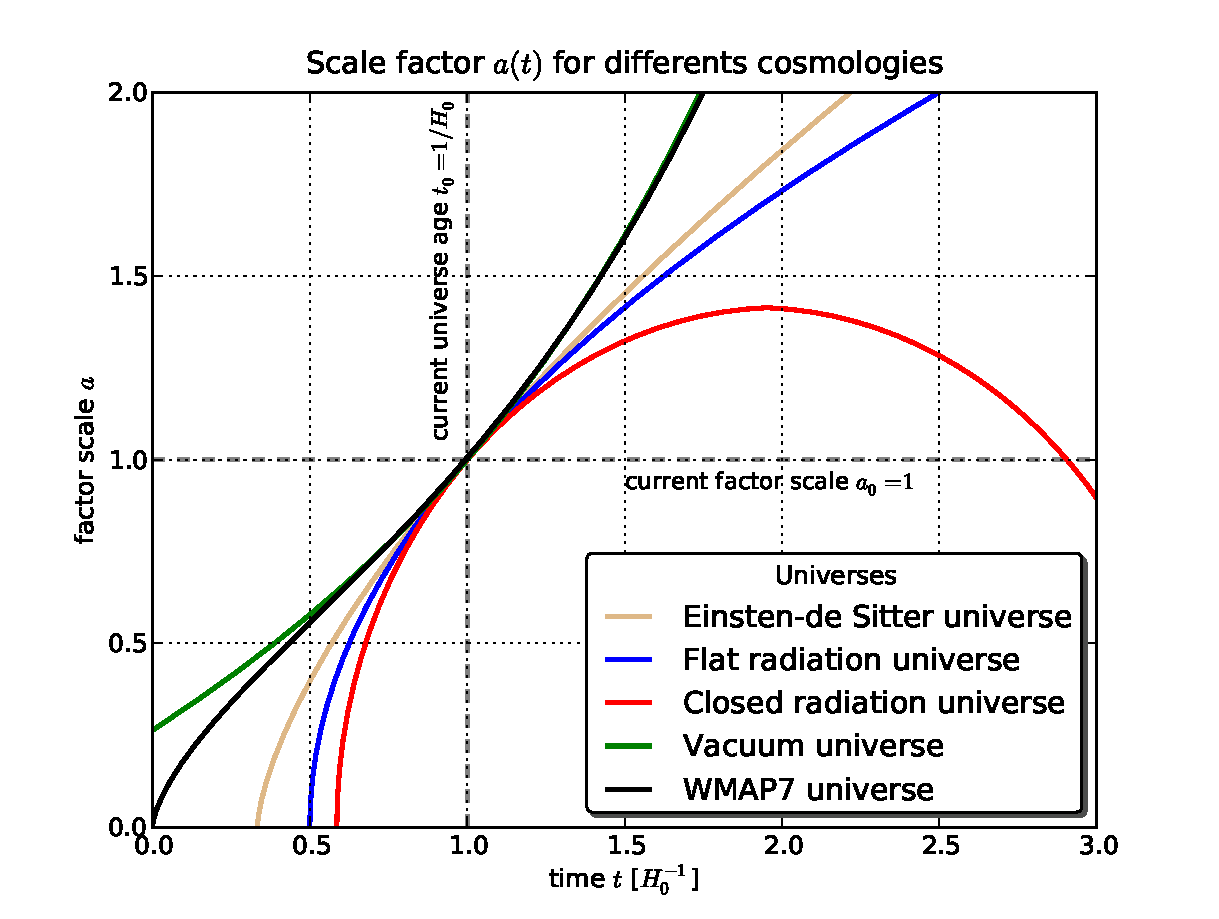
\includegraphics[trim = 12mm 4mm 17mm 8mm, clip, keepaspectratio=true,
  width=0.4\textheight]{./figures/Friedmann_Solution.pdf}
  
  \caption{\small Different solutions to the Friedmann's equation. The WMAP7
  solution is consistent with our Universe, where the current epoch
  is vacuum dominated, corresponding with an accelerated expansion.}

  \label{fig:Friedmann}

\end{figure}
%.........................................................................


Nevertheless, an uniform fluid model cannot account for the bound structures 
observed at smaller scales like galaxies and clusters. It is hence necessary 
to modify the Friedmann's solutions in order to include small perturbations 
that enable the evolution of such a bound structures at the current time. To do
so, the Einstein's equation is linearized as follows \citep{padmanabhan1995}:


\eq{LinearEinstein}
{ \mathcal{L}(R_{\mu \nu}, \delta R_{\mu \nu}) = \frac{8\pi G}{c^2}
( T_{\mu \nu} + \delta T_{\mu \nu} ) }


This approach can be demonstrated to be equivalent to introducing basic 
Newtonian fluid equations for the matter component.

%.........................................................................	
%Fluid Equations
\begin{eqnarray}
%.........................................................................	
\label{eq:ContinuityEquationC}
\matrix{\mbox{\footnotesize{Continuity}} \cr \mbox{\footnotesize{equation}}} & &
\der{\delta}{t} = - \frac{1}{a}\nabla_r \cdot \corc{ (1+\delta)\bds v }\\
\nonumber{}
\\
%.........................................................................	
\label{eq:EulerEquationC}
\matrix{\mbox{\footnotesize{Euler's}} \cr \mbox{\footnotesize{equation}}} & &
\der{\bds v}{t} + \frac{\dot a}{a}\bds v + 
\frac{1}{a}\pr{ \bds v\cdot \nabla_r }\bds v = 
-\frac{\nabla_r P}{a \bar \rho(1+\delta)} - 
\frac{1}{a}\nabla_r \Phi \\
\nonumber{}
\\
%.........................................................................	
\label{eq:PoissonEquationC}
\matrix{\mbox{\footnotesize{Poisson's}} \cr \mbox{\footnotesize{equation}}} & &
\nabla^2_r \Phi = 4\pi G\bar \rho a^2 \delta
\end{eqnarray}
%.........................................................................	
where $\rho = \bar\rho + \delta \rho = \bar \rho (1+\delta)$ is the matter 
density, $\bds v$ is the peculiar velocity, $\Phi = \phi + \ddot a a r^2/2$ 
the peculiar gravitational potential, $P$ the fluid pressure and all gradients 
are evaluated in comoving coordinates.

\

Assuming an equation of state for an inviscid gas and decomposing the density 
field into Fourier modes (for a flat universe), we obtain:


\eq{ContinuityEquationCMode}
{ \dtot{^2 \delta_{\bds k}}{t^2} + 2\frac{\dot a}{a}\dtot{\delta_{\bds k}}{t} =
\corc{ 4\pi G \bar \rho - \frac{c_s^2}{a^2}k^2 }\delta_{\bds k} }
where $\delta_{\bds k}$ are the modes of the density and $c_s$ the velocity of 
the sound in the medium. For the linear regime, where perturbations are still
valid, each mode evolves independently. It is hence possible to assume a general
solution of the form $\delta_{\bds k}(t) = \delta_{\bds k}(0) D(t)$, where $t=0$ 
is referred to as some suitable time after the epoch of recombination and $D(t)$
is the linear growth function, given by:

\eq{LinearGrowth}
{ D(a) = \frac{5}{2}\Omega_m\corc{ \Omega_m^{4/7} - \Omega_\Lambda + 
\pr{ 1+\frac{\Omega_m}{2} }\pr{ 1+\frac{\Omega_\Lambda}{70} } }^{-1} }

At this point, it is possible to follow completely the evolution of the Universe
in the linear regime. However, when the modes of the density field become large
enough $\delta\gg 1$, the assumption of independence is not longer adequate, it 
is hence necessary to evaluate numerically the evolution in the non-linear 
regime.

%.........................................................................
%FIGURE 2: Zel'dovich approximation
\begin{figure}[h]
\centering

  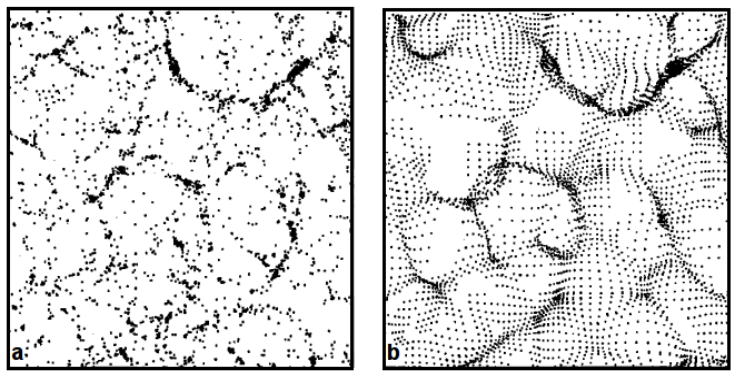
\includegraphics[trim = 0mm 0mm 0mm 2mm, clip, keepaspectratio=true,
  width=0.4\textheight]{./figures/Zeldovich_Approximation.png}
  
  \caption{\small Comparison of the evolution of a density field for a 
  N-body simulation (left) and for the Zel'dovich approximations (right).
  Taken from \cite{longair2008}.}

  \label{fig:Zeldovich}

\end{figure}
%.........................................................................

In order to provide a set of initial conditions for numerical runs, it can be 
used the Zel'dovich approximation \citep{Zeldovich70}. This approximation allows
to follow the evolution of primordial perturbations in the quasi-linear regime 
($\delta \sim 1$), what makes it very suitable to tie analytical solutions in 
the linear regime with numerical solutions in the non-linear regime. Using the
Lagrangian frame and taking certain portion of the fluid, its trajectory can 
be described as follows:

\eq{Zeldovich}
{ \bds r(t,\bds q) = a(t)\corc{ \bds q + \bds{\Psi}(\bds q, t) } }

where $\bds q$ is the comoving Lagrangian coordinate when fluid is not 
perturbed and $\bds{\Psi}(\bds q, t)$ is the displacement function that 
accounts for clustering. The displacement function can be approximated as 
$\bds{\Psi}(\bds q, t) = D(t)\bds{\Psi}(\bds q)$, where $D(t)$ is the linear 
growth function [Eq. \ref{eq:LinearGrowth}] and $\bds{\Psi}(\bds q)$ is given 
by:

\eq{Displacement}
{ \bds{\Psi}(\bds q) = \int \frac{d^3 k}{(2\pi)^3}e^{i \bds k \cdot \bds q}
\frac{i\bds k}{k^2}\delta_{\bds k}(0) }

In this same fashion, the perturbed velocity field can be constructed by means
of the Zel'dovich approximation. Then, discretizing the fluid, it is obtained a 
set of positions and velocities $\{\rho_i,\bds r_i, \bds v_i\}$ corresponding 
with the input initial conditions for some numerical scheme for evolving the 
non-linear regime, like \SPH, \VPH, \AMR.


\subsection*{Smoothed Particle Hydrodynamics (SPH)}
As was previously discussed, the dark matter component of the Universe can be 
modelled as an inviscid and collisionless gas whereas the baryonic component as 
a collisional and dissipative gas, both following the standard fluid equations 
[\ref{eq:ContinuityEquationC}], [\ref{eq:EulerEquationC}], 
[\ref{eq:PoissonEquationC}].The objective of any hydrodynamic scheme is then 
solving these set of equations in a suitable way. One of the classic schemes 
widely used by the astrophysical community for this task is the Smoothed 
Particle Hydrodynamics \SPH\ as introduced by \citet{Lucy77} and 
\citet{Gingold77}. \SPH\ solves the continuous dynamic of the fluid by first
discretizing it into parcels, where each of these parcels samples the properties 
of the fluid. The evolution is reached by solving the equations of motion
directly over the moving particle-parcels. Finally, the continuous properties 
of the gas are recovered by means of interpolation techniques.

\subsubsection*{Kernel Interpolants}

The core of \SPH\ is the kernel interpolant formalism, where a continuous field 
can be recovered from a discrete set of sampling particles. For any physical 
field $F(\bds r)$ it may be defined a smoothed version $F_s(\bds r)$ as

\eq{SmoothedF}
{ F_s(\bds r) = \int_V \bds F(\bds r')W(\bds r - \bds r'; h) d\bds r' }
where the integral extends over the volume domain and $W(\bds r;h)$ is the 
kernel interpolant, with $h$ being the smoothing length, related to the 
integration volume and the kernel domain. 

\

Several different expressions for the kernel can be used for obtaining the 
smoothed versions of the fields, where the only conditions to satisfy are 
normalization $\int W(\bds r; h)d\bds r= 1$ and convergence to the Dirac delta 
when $h\rightarrow 0$. Nevertheless, finite-range kernels like the cubic spline 
kernel are preferred for their compact support and their easy computational 
implementation.

\eq{kernel}
{ W(r; h) \equiv W\pr{ \frac{r}{2h} } = W(q) = \frac{8}{\pi}
\left\{ \matrix{ 1-6q^2 + 6q^3, & 0 \leq q \leq 1/2, \cr
2(1-q)^3, & 1/2 < q \leq 1,\cr
0, & q>1 } \right. }

If we fix the masses of the sampling particles to be $\{m_i\}_i$, the volume
element of each may be approximated as $\Delta \bds r_i = m_i/\rho_i$. The 
variation of the volume hence relies on the variation of the density. The 
integral shown in [\ref{eq:SmoothedF}] can be then approximated as

\eq{DiscreteF}
{ F'_i \equiv F_s(\bds r_i) \approx \sum_j^{N_{tot}} \frac{m_j}{\rho_j}F_j 
W(\bds r_i - \bds r_j; h_i) }
here we use the notation $F'_i = F_s(\bds r_i)$ for the smoothed fields and $F_i 
= F(\bds r_i)$ for the original fields. Although smoothed fields are defined
for any position, we are just interested in the positions of the sampling 
particles $\{r_i\}$. Note that the summation runs over all particles, however, 
due to the finite-range kernel adopted, it is reduced only to the neighbours 
inside a sphere of radius $2h$. Hereafter, the smoothing lengths will be taken 
as adaptive for each particle, what is necessary in order to keep a good 
precision for high density contrasts occurring in many astrophysical situations.

\

One of the main appealing of the kernel interpolant formalism of \SPH\ is the
handling of differential operators, where the conditions of continuity and 
differentiability relies on the kernel rather than the field itself. This is 
advantageous when dealing with sparse distributions or very rugged fields. So
we obtain:

\eq{DiffField}
{ \mathcal{D}_i[F_s(\bds r_i)] = \sum_j^{N_{tot}}\frac{m_j}{\rho_j}F_j 
\mathcal{D}_i[W(\bds r_i - \bds r_j; h_i)] }
where $\mathcal{D}_i$ is any differential operator evaluated at $\bds r_i$. Note
that this expression includes the possibility of $h_i$ as a function of the 
coordinates, which is the more general case. A very useful expression is the 
divergence of the velocity field, yielding

\eq{DivV}
{ (\nabla \cdot \bds v)_i = \frac{1}{\rho_i}\sum_j^{N_{tot}} m_j (\bds v_j - \bds v_i)
\cdot \nabla_i W(\bds r_i - \bds r_j; h_i) }
where vectorial identities have been used in order to symmetrize the expression.

\subsubsection*{Equations of Motion}

Once discussed the kernel interpolant formalism, we proceed to describe how to
get the equations of motion to be solved computationally. The original approach
consists in dealing directly with differential operators of the fluid equations 
[\ref{eq:ContinuityEquationC}], [\ref{eq:EulerEquationC}], 
[\ref{eq:PoissonEquationC}] according to the equation [\ref{eq:DiffField}] 
\citep{Lucy77,Gingold77}. Instead, we will take the approach first proposed by 
\citet{Gingold82} and further developed by \citet{Springel11}. This consists of 
a variational derivation of the equations of motion by first discretizing the 
Lagrangian of the system. The main advantage of this derivation is that it 
retains the conservation laws associated to the Hamiltonian dynamics in a 
natural fashion.

\

As demonstrated by \citet{Eckart60}, the hydrodynamic equations can be derived
from the Lagrangian

\eq{LagrangianFluid}
{ \mathcal{L} = \int \rho \pr{ \frac{v^2}{2} - u }dV }
where $u$ carries with all the interactions of the system. Using the kernel 
interpolant formalism, we can rewrite this expression as

\eq{LagrangianDiscrete}
{ \mathcal{L} = \sum_i \pr{ \frac{1}{2}m_i v_i^2 - m_i u_i } }

For an inviscid gas, the equation of state is given by

\eq{EOSgas}
{ u_i(\rho_i) = A_i\frac{\rho_i^{\gamma-1}}{\gamma-1} = 
\frac{P_i}{\rho_i}\frac{1}{\gamma-1} }
where $\gamma$ is the adiabatic index, $A_i$ the specific entropy and $P_i$ the
pressure as evaluated in the $i$th particle. Introducing this expression into
the Lagrangian [\ref{eq:LagrangianDiscrete}], considering the implicit of the
smoothing length with the coordinates and applying the Euler-Lagrange equations,
it is obtained the equations of motion:

\eq{EoMIdeal}
{ \frac{d\bds v_i}{dt}= -\sum_{j=1}^N m_j \corc{ f_i\frac{P_i}{\rho_i^2}\nabla_i
W_{ij}(h_i)+f_j\frac{P_j}{\rho_j^2}\nabla_i W_{ij}(h_j)} }
where the coefficients $f_i$ are defined as:
\[ f_i = \corc{ 1+\frac{h_i}{3\rho_i}\frac{\partial \rho_i}{\partial h_i} }^{-1} \]

The estimation of the smoothing length of each particle is reached through the
implicit differentiation of the expression $\rho_i h_i^3 = const$, what 
guarantees a mass conservation inside the volume of the kernel.

\

Although this equation of motion follows the evolution of an inviscid gas, what
is a very approximate description of the matter in a cosmological setup, there
are some problematic situations where the approximation is not longer suitable.
Namely shock dynamics, where the strict entropy conservation would generate
undesirable oscillations. It is hence necessary to introduce a new term that 
accounts for entropy dissipation in shocks but keeping the inviscid dynamics of
the gas elsewhere. This new term, so-called artificial viscosity, is introduced 
in the form or a extra term in the equation of motion as

\eq{ViscosityTerm}
{ \left. \frac{d \bds v_i}{dt}\right|_{\mbox{\footnotesize visc}} =
- \sum_{j=1}^N m_j \Pi_{ij}\nabla_i \overline{W}_{ij} }
where $\Pi_{ij}$ is the viscous tensor and $\overline{W}_{ij} = [W_{ij}(h_i)+
W_{ij}(h_j)]/2$. Throughout the literature may be found several different 
parametrizations of the viscous tensor, however the standard parametrization
proposed by \citet{Monaghan83} has demonstrated to be very adequate.

\eq{ViscousTensor}
{ \Pi_{ij} = \left\{ \matrix{ \corc{-\alpha c_{ij}\mu_{ij} + \beta \mu_{ij}^2}/\rho_{ij} & 
\mbox{if} \bds v_{ij}\cdot \bds r_{ij} <0 \cr 0 & \mbox{otherwise}}\right. }
with $\mu_{ij}$ defined as

\[ \mu_{ij} = \frac{h_{ij}\bds v_{ij}\cdot \bds r_{ij}}{|\bds r_{ij}|^2 + 
\epsilon h_{ij}^2} \]
where $h_{ij}$, $\rho_{ij}$ and $c_{ij}$ are the arithmetic means of the smoothing
length, the density and the sound speed of the $i$th and the $j$th particles 
respectively. The softening parameter $\epsilon$ is introduced in order to avoid
divergence when two particles come very close to each other. The parameters 
$\alpha$ and $\beta$ quantify the strength of the viscosity term when activated.
Usually they are chosen to be $\alpha \approx 0.5-1.0 $ and $\beta=2\alpha$.

\

Note that this viscous term is only activated when two particles come rapidly 
close to each other, what is caused in most cases by a shock. The entropy 
generated in this way is always positive definite, accounting for the required
dissipation in shocks.

\

As we are interested in astrophysical applications, it is clear the necessity 
of coupling self-gravity to the equations of motion derived for \SPH. Instead 
of taking the previous approach for the viscous term, we shall couple the
self-gravity by first introducing an associated Lagrangian term that will
ensure the energy conservation when gravity is included.

\eq{LagrangianG}
{ \mathcal{L}_g = -\frac{G}{2}\sum_{i\neq j}m_im_j \phi( r_{ij}, \epsilon_j ) }
where the gravitational potential $\Phi(\bds r)$ has been defined as 
$\Phi(\bds r) = G \sum_i m_i \phi(\bds r - \bds r_i, \epsilon_i)$, and $\epsilon_i$
is a softening parameter introduced to prevent singularities. Applying the 
Euler-Lagrange equations, we obtain the next equation of motion for the 
gravitation:


\eq{GravityTerm}
{ \left.\frac{d \bds v_i}{dt}\right|_{\mbox{\footnotesize{grav}}} = 
-\sum_j Gm_j \frac{\bds r_{ij}}{r_{ij}}\frac{[\dot\phi(\bds r_{ij},\epsilon_i)+
\dot\phi(\bds r_{ij},\epsilon_j)]}{2} - \frac{1}{2}\sum_{j\neq k}G\frac{m_jm_k}{m_i}
\frac{\partial \phi(r_{jk}, \epsilon_j)}{\partial \epsilon}\frac{\partial \epsilon_j}
{\partial \bds r_i} }


In this equation we have enabled an adaptive softening length depending on each 
particle position, this is necessary in order to gain a better numerical 
convergence. One way of estimating this parameter is to related it directly with
the smoothing length of the kernel, i.e. $\epsilon_i = \epsilon_i(h_i)$. It is 
also noteworthy that these summations run all over the sampling particles as the 
kernel is not involved, so summations are not restricted only to nearby neighbours. 
This requires the implementation of sophisticated gravity solvers in order to 
avoid the prohibitive computing time scaling as $\mathcal{O}(N^2)$. Several 
gravity solver may be found in the literature, however the \texttt{TreeCode} 
algorithm by \citet{barnes1986} scaling as $\mathcal{O}(N\log N)$ has been widely 
used for this purpose.

\

Finally, the evolution of the fluid is reached by solving numerically the 
differential equations leaded by the inviscid, the viscous and the gravitational 
terms and taking the initial conditions provided by the Zel'dovich approximation. 
In order to do so, some numerical integration scheme has to be adopted, namely a 
symplectic integrator or even a time integrator scheme like Runge-Kutta.


\subsection*{Voronoi Particle Hydrodynamics (VPH)}

Although \SPH\ is very versatile for a variety of fluid problems and the
computational implementation is direct due to its Lagrangian nature, the density
estimation based on the kernel interpolant formalism exhibits some problems. 
Namely \SPH\ fails in recovering the total volume, i.e. the sum of all the 
volume elements of the sampling particles is not equal to the volume of the
simulation, and the smoothing of the density field across contact discontinuities
generates non-desirable spurious suppressions.

\

Several modifications of the original formulation of \SPH\ have been proposed in
order to improve the accuracy. Among them is very interesting the one proposed 
by \citet{Hess10}, in which is introduced a new estimative of the density field 
based on a Voronoi tesellation of the sampling particles. Tessellations 
techniques have been previously introduced as estimators of physical fields in
simulations (see e.g. Delaunay Tessellation Field Estimator DTFE by 
\citet{Schaap00}) with more accurate results than kernel interpolants of \SPH\
\citep{Pelupessy03}.

\
%.........................................................................
%FIGURE 3: Tesselations
\begin{figure}[h]
\centering

  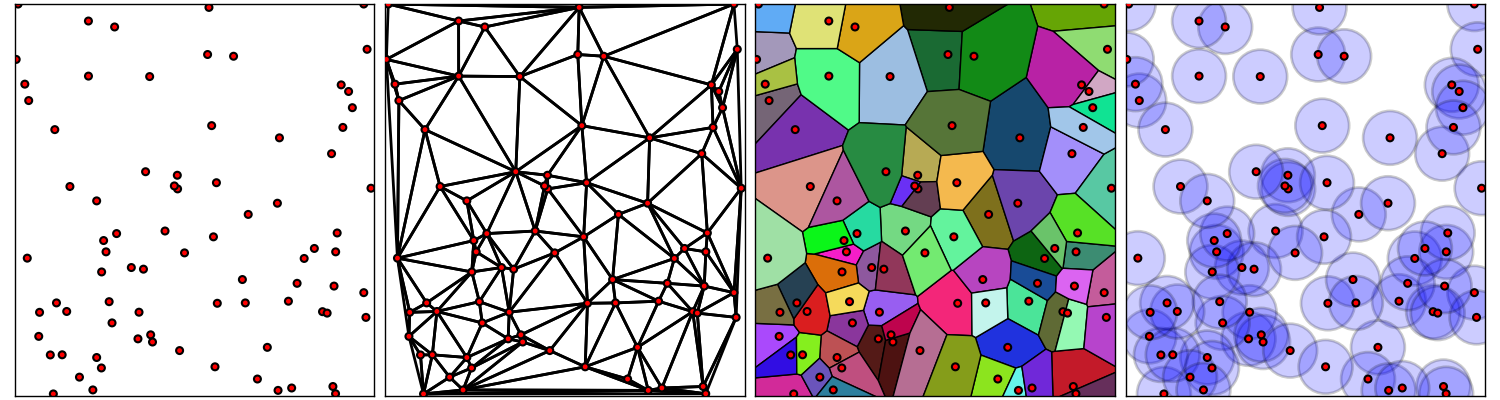
\includegraphics[trim = 0mm 0mm 0mm 0mm, clip, keepaspectratio=true,
  width=0.7\textheight]{./figures/Tessellations.png}
  
  \caption{\small Estimation techniques of the density field. Original 
  dataset (first). Delaunay tessellation (second). Voronoi tessellation 
  (third). Spherical kernel volumes (fourth). }

  \label{fig:Tessellations}

\end{figure}
%.........................................................................

Although Delaunay tessellation was first introduced for field estimation, it 
exhibits some problems that makes it unsuitable for some pathological 
situations. Due to the definition of a Delaunay triangulation, where no point 
of the dataset must be inside the circumcircle of any triangle of the 
tessellation (see Fig. \ref{fig:Tessellations}), there may be more than a 
triangulation for a same dataset, besides the volumes of the polyhedra do not 
change continuously with the coordinates of the particles as they evolve, 
generating non-desirable discontinuities in the hydrodynamical equations.

\

A Voronoi tessellation is defined as a set of adjacent polyhedra outlined by
the bisector planes of neighbour points of the dataset (see Fig. 
\ref{fig:Tessellations}). This definition makes unique the tessellation 
associated to a dataset and does not generate discontinuities in the 
estimations. For these reasons, the Voronoi tessellation is preferable for 
field estimation in the context of hydrodynamics, as established by 
\citet{Hess10}.


\subsubsection*{Equations of Motion}

Starting from the discretized Lagrangian [\ref{eq:LagrangianDiscrete}] and 
applying Euler-Lagrange variational equations, we obtain:

\begin{eqnarray}
\nonumber{}
m_i \frac{d \bds v_i}{dt} &=& - \sum_j m_j \frac{\partial u_j}{\partial \bds r_i} \\
\label{eq:VPHLarangian}
&=& -\sum_j m_j \frac{P}{\rho_j^2}\frac{\partial \rho_j}{\partial V_j}\frac{\partial V_j}{\partial \bds r_i}
\end{eqnarray}
where has been used the equation of state of an inviscid gas and the variation
of the density has been relied on the variation of the volume of the Voronoi 
polyhedron $V_j$ associated to the $j$th particle. The first derivative term has 
to be computed through some estimation of the density field, the simplest one and 
usually adopted is 

\eq{DensityEstimation}
{ \rho_i= \frac{m_i}{V_i} }

%.........................................................................
%FIGURE 4: Voronoi Volume
\begin{figure}[h]
\centering

  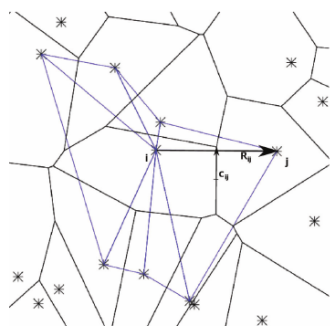
\includegraphics[trim = 0mm 0mm 0mm 0mm, clip, keepaspectratio=true,
  width=0.25\textheight]{./figures/VoronoiVolume.png}
  
  \caption{\small It is sketched how to evaluate the dependence of the volume
  of a Voronoi cell on the coordinates of neighbour particles (asterisks). 
  Vectors $\bds c_{ij}$ and $\bds e_{ij}$ needed to calculate the derivative
  are also sketched. Taken from \citet{Hess10}. }

  \label{fig:VoronoiVolume}

\end{figure}
%.........................................................................

The evaluation of the second derivative term can be reached by means of a 
geometric analysis \citep{Serrano01}, yielding:

\begin{eqnarray}
\nonumber{}
\frac{\partial V_j}{\partial \bds r_i} &=& -A_{ij}\pr{ \frac{\bds c_{ij}}{R_{ij}}
+ \frac{\bds e_{ij}}{2} } \ \ \ \ \mbox{for}\ \ \ i\neq j \\
\label{VoronoiVolume}
\frac{\partial V_j}{\partial \bds r_i} &=& -\sum_{k\neq j}\frac{\partial V_k}{\bds r_i} \ \ \ \ \mbox{for}\ \ \ i=j
\end{eqnarray}
where $\bds e_{ij} = (\bds r_j - \bds r_i )/R_{ij}$ is a unitary vector 
pointing from the $i$th particle to the $j$th neighbour, $A_{ij}$ is the area 
of the Voronoi face between the cells $i$ and $j$, and $\bds c_{ij}$ is defined
as sketched in Fig. \ref{fig:VoronoiVolume}. The expression when $i=j$ is 
obtained by invoking volume conservation.

\

Finally, the equation of motion for an inviscid gas is given by

\eq{VoronoiEoM}
{ m_i \frac{d \bds v_i}{dt} = - \sum_{i\neq j}^N A_{ij}\corc{ 
(P_i+P_j)\frac{\bds e_{ij}}{2}+(P_j-P_i)\frac{\bds c_{ij}}{R_{ij}} } }
where the right hand term has been explicitly symmetrized. It is noteworthy that
the summation only runs over neighbour cells as the area of the face $A_{ij}$ 
vanishes for non-abutted cells. Unlike kernel interpolants, where the number of
contributing terms of the summation depends on the user-defined smoothing 
length of the kernel, Voronoi tessellations restricts naturally this number, 
depending only on the number of faces of the Voronoi cell.

\

Although the Voronoi tessellation estimator improves greatly the efficiency of 
\SPH, it is still required to use a viscous term in order to account for shock
dynamics. As the expression [\ref{eq:ViscosityTerm}] for \SPH\ involves the kernel
interpolant, it is necessary to introduce a new form of the viscous term that 
can work with \VPH. Here we adopt the parametrization of \citet{Hess10}, 
yielding:

\eq{ViscosityTermVPH}
{ \left. m_i\frac{d \bds v_i}{dt}\right|_{\mbox{\footnotesize visc}} =
- \sum_{j=1}^N A_{ij} {\rho}_{ij}^2\Pi_{ij}\frac{\bds e_{ij}}{2} }
$\rho_{ij}$ is the arithmetic mean of the densities of the $i$th and the $j$th 
particles and the viscous tensor is given by:

\eq{ViscousTensorVPH}
{ \Pi_{ij} = \left\{ \matrix{ \corc{-\alpha c_{ij}w_{ij} + \beta w_{ij}^2}/\rho_{ij} & 
\mbox{if} \bds v_{ij}\cdot \bds r_{ij} <0 \cr 0 & \mbox{otherwise}}\right. }
where $w_{ij}$ is the projected pairwise velocity defined as

\[ w_{ij} = \frac{ \bds v_{ij}\cdot \bds r_{ij} }{|\bds r_{ij}|} \]

Note that this definition of the viscous tensor is exactly equal to the adopted 
for \SPH, but changing $\mu_{ij}$ for $w_{ij}$ as the parameter $\mu_{ij}$ 
depends on the smoothing length of the kernel. The parameters $\alpha$ and 
$\beta$ are chosen like \SPH, i.e. $\alpha \sim 0.5-1.0$ and $\beta = 2\alpha$.

\

Finally, for the self-gravity term, note that Eqs. [\ref{eq:LagrangianG}] and 
[\ref{eq:GravityTerm}] do not involve the kernel at all, and the summation runs
all over the sampling particles. This implies that this term remains equal for 
\VPH, and the same gravity solver techniques previously discussed for \SPH\ are
equally applicable here.

%==============================================================================
\section{Methodology}
%==============================================================================
The proposed project is subject to a M.Sc. study and will cover the following 
steps:


\begin{itemize}
\item[\checkmark] \textit{First, a bibliographic review of the original papers 
of the discussed methods will be done. Also a review of previous comparison 
projects.}
\end{itemize}


Before carrying out our enterprise in quantifying the performance of \VPH\ over
cosmological setups, it is necessary to understand deeply the foundations of 
the classic approaches. At this point, a detailed bibliographic review of the 
original papers (for \SPH, \AMR, \VPH\ and \AREPO) should be done. Although no 
previous works have been done in comparing thoroughly the performance of \VPH\
with other approaches over cosmological setups, there are a plenty of comparison
projects for the classic approaches and even \AREPO\ over galaxy simulations and 
commonly used benchmark problems. This literature will have to be reviewed as 
well.

\

\begin{itemize}
\item[\checkmark] \textit{Second, a design of the numerical experiments should 
be done at this point. This includes making cosmological simulations using 
different techniques and if necessary, constructing and simulating specific 
benchmark problems.}
\end{itemize}


As this project will be entirely based on numerical results, computing a set of
cosmological simulations as well as some benchmark problems is one of the key 
steps. For this purpose, we will use some packages like \texttt{GADGET} 
\citet{Springel05} for \SPH\ simulations, \texttt{RAMSES} \citet{Teyssier02} 
for \AMR\ and a modified version of \texttt{GADGET} for \VPH. Other standard 
benchmark problems will be also simulated, e.g. the sod shock tube, 
Kelvin-Helmholtz instabilities, a gas cloud in a supersonic wind.

\

\begin{itemize}
\item[\checkmark] \textit{Third, a thorough analysis of the numerical results 
will be done.}
\end{itemize}


Once obtained the numerical results from the performed simulations, a thorough
analysis of the physical accuracy of \VPH\ as compared with the other techniques
will be done for each situation. A computational performance analysis of the 
\VPH\ technique will be also carried out, i.e. computing time, memory and 
processor usage.

\

\begin{itemize}
\item[\checkmark] \textit{Fourth, a first-author paper with the main result will
be prepared.}
\end{itemize}


The more relevant results of our project will be prepared as a paper and 
submitted to some high impact international journal. If possible, a participation
in some international event is also included in this step.

\

\begin{itemize}
\item[\checkmark] \textit{Fifth, a thesis will be written.}
\end{itemize}


A dissertation for obtaining a M.Sc. in Physics degree will be prepared. A
streamlined description of each technique will be included as well as the 
presentation of the performed simulations and a discussion of all our results
and conclusions.


%==============================================================================
\section{Previous Experience}
%==============================================================================
Previous activities and projects related with Numerical Cosmology have been 
successfully carried out within the FACom group, many of these leaded by Prof. 
Juan Carlos Munoz-Cuartas. This demonstrates the broad research expertise of the 
supervisor in the topic and the availability of computational resources (computing
time, software) required to perform this project satisfactorily.

\

On the other hand, at the present the student has already some of the fundamental 
knowledge in Astrophysics and Cosmology required for this investigation. This can 
be confirmed by his research experience, including a paper (as co-author) 
published in the ApJL in which the kinematics of the Local Group in a cosmological 
context was studied, another paper (as co-author) published in the ApJ where the 
influence of thermal evolution on the magnetic habitability of rocky planets was 
studied, and some participations in academic congresses. Furthermore, a Bachelor’s 
thesis where the preferred place of simulated Local Group-like systems in the 
cosmic web was studied, also demonstrates the ability of the applicant for 
handling simulations and massive data, a skill that is necessary for carrying out 
this project.

\

Finally, it is worth mentioning the ongoing and already done work related with 
this project. First, the required codes for performing our simulations are already
available (including a modified version of \texttt{GADGET} for \VPH). Some
cosmological simulations have been performed as well. Furthermore, part of the 
toolbox of codes for our analysis has been already developed\footnote{You can 
find some codes and further information of the present stage of the project in 
this repository \url{https://github.com/sbustamante/MethodsComparison}}, 
including basic miscellaneous functions for handling data, plotting point 
distributions and constructing phase diagrams.


%==============================================================================
\section{Scientific Impact}
%==============================================================================
The matter content of the Universe has been probed to be dominated by the dark 
matter component \citep{Planck13XVI}. Accordingly, most of the related numerical 
work in cosmology and galaxy formation has been carried out based on dark matter 
only simulations. Nevertheless, on smaller (galactic) scales, the effects of 
baryons become significant. For example, recent hydrodynamical simulations show 
that filamentary gas accretion in early stages of galaxy evolution is a key 
physical process; there is evidence that it plays a central role in the formation 
of discs \citep{Dubois14}, determining the alignment of galaxies with respect to 
the web \citep{Hahn10} and fuelling high star formation rates \citep{Dekel09}.

\

These results show the importance of modelling baryons by incorporating gas 
dynamics into cosmological simulations. For this purpose, \AMR\ and \SPH\ have
been widely used by the astrophysical community. However, due to the singular 
situations where each of those techniques fails, general purpose hydrodynamical
simulations cannot be reached by means of them.

\

The recently developed approach \AREPO\ \citet{Springel10} has demonstrated to 
be highly efficient dealing with some of the most critical weaknesses of \AMR\ 
and \SPH, what makes it a very appealing alternative. However, its demanding 
computing time also makes it infeasible when computational resources are rather 
limited. In this direction, our endeavour in quantifying the computational 
performance and the improved physical accuracy of \VPH\ would contribute with 
valuable insight of this technique as a more feasible option when limited 
computational resources are available.


%==============================================================================
\section{Expected Results}
%==============================================================================
At the end of the stipulated development time for this project, we hope to have
obtained the following results:
\begin{itemize}
\item A toolbox of codes to study the performance of hydro-solvers over 
cosmological setups and over standard benchmark problems in fluid mechanics.
\item A set of cosmological simulations computed by using each of the studied
techniques.
\item A M.Sc. thesis.
\item Submitting a first-author paper to an international journal.
\item Participating with a poster or an oral presentation in an international
event.
\end{itemize}


%==============================================================================
\section{Schedule}
%==============================================================================
Next it is shown a table with the proposed activities scheduled for each term.

\begin{table}[h]
\begin{flushleft}
\begin{center}
  \begin{tabular}{l  c c c c } \hline\hline
	\centering\textbf{Goals} & \textbf{Term I} & \textbf{Term II} & 
	\textbf{Term III} & \textbf{Term IV} \\ \hline\hline
	
	 Bibliographic review & X & & & \\
	 Numerical experiments & X & X & & \\
	 Analysis of results &  & X & X & \\
	 International journal paper &  &  & X & \\
	 Dissertation &  &  &  & X \\
	\hline\hline
  \end{tabular}  
  \caption{ Terms range from 2014-02 for term I, up to 2016-01 for term IV.}
\end{center}
\end{flushleft}
\end{table}


%==============================================================================
\bibliographystyle{latex/mn2e}
\renewcommand{\bibname}{11\ \ \ \ Bibliography}
\small
\bibliography{references.bib}
%==============================================================================

\end{document}